\documentclass[UTF8]{article}
\usepackage{geometry}
\usepackage{mathrsfs,amsmath}
\usepackage{amssymb}
\usepackage{mathbbol}
\usepackage{enumerate}
\usepackage{needspace}
\usepackage{graphicx}
\graphicspath{{./images}}
\newcommand{\mycite}[1]{\textbf{\textit{#1}}}
\newcommand{\opinion}[5]{$\omega_{#1} = (#2, #3, #4, #5)$}
\begin{document}
    
\title{COMP 8920 - Computational Reasoning in AI \\Midterm}
\author{
    Vijay Rajasekar Thirulokachander \\
    \large 105092311 \\
    \large thirulo@uwindsor.ca
}
\maketitle
\date{}


\section{Binary Division Constraint Derivation}
\section{Defintions of concepts and their applications in reasoning}
\subsection{Probability Measure}

Out of the many approaches to represent belief and uncertainty, probability has the advantage of being well understood.  It is a powerful tool; many technical results have been proved that facilitate its use, and a number of arguments suggest that, under certain assumptions (whose reasonableness can be debated) probability is the only “rational” way to represent uncertainty. [Lecture Slides 1B]\\

Consider now a completely arbitrary nonempty set of possible outcomes to be $\Omega$ . A class $\mathcal{F}$ of
subsets of $\Omega$ is called a field if it contains $\Omega$ itself and is closed under the
formation of complements and finite unions: 
\begin{enumerate}[i]
    \item $ \Omega \in \mathcal{F}$
    \item $A \in \mathcal{F} $ implies $\neg A \in \mathcal{F}$ 
    \item $ A, B \in \mathcal{F}$ implies $A \cup B \in \mathcal{F}$
    
\end{enumerate}
A set function is a real-valued function defined on some class of subsets of
$ \Omega $. A set function P on a field  $ \mathcal{F}$ is a \textit{probability measure} if it satisfies these
conditions:
\begin{enumerate}[i]
    \item $ 0< P(A)< 1 $ for $ A \in \mathcal{F} $
    \item $ P(\emptyset) = 0, P(\Omega) = 1 $
    \item if $ A_1, A_2, ... $ is a disjoint sequence of $ \mathcal{F} $ sets and if $ \cup^\infty_{k=1} \in \mathcal{F}$ i.e the union of all sequences of $\mathcal{F} $ sets belongs to $\mathcal{F}$ then
    $$ P \left( \bigcup_{k = 1}^{\infty} A_k \right) = \sum_{k=1}^{\infty} P(A_k) $$ i.e the probability of the union of all disjoint sequences is equal to the sum of probability of each disjoint sequence. This property is referred to as \textit{finite additivity}.
\end{enumerate}
The above definitions were obtained from the book \mycite{Probability and Measure, Third Edition, Patrick Billingsley, Pg. 19 - 23}

[https://www.colorado.edu/amath/sites/default/files/attached-files/billingsley.pdf] \\

Sets of probability measures have many of the advantages of probability, and may be more appropriate in a setting where there is uncertainty about the likelihood.  Considering sets of weighted probability measures allows for more flexible modeling, but has the disadvantage of needing yet more numbers to characterize a situation.

\subsection{Belief Function}
Belief in a set of elements, say A, of a frame $\theta$, represents the total belief that one has
based on the evidence obtained. It is the sum of all the belief masses assigned to elements that
are contained in the set A and the belief mass assigned to the set A. Mathematically, one can
express the total belief in the set A as $$ Bel(A) = \sum_{B \subseteq A} m(B) $$ Unlike probability theory, Bel(A) = 0
represents lack of evidence about A, while P(A) = 0 represents the impossibility of A. However,
Bel(A) = 1 represents certainty, that is A is certain to occur, similar to P(A) = 1, which also
represents the certainty that A is true. \mycite{[Srivastava, Rajendra P.. “The Dempster-Shafer Theory of Belief Functions for Managing Uncertainties : An Introduction and Fraud Risk Assessment Illustration 1.” (2012).]}

Prof. Judea Pearl, in his work \mycite{Reasoning with Belief Functions: An Analysis of Compatibility}, provides three domains of reasoning in which belief functions are applied:
\begin{enumerate}[i]
    \item \textit{Representation of incomplete knowledge}: In cases where fully specified
    probabilistic knowledge is not available, belief functions are often used to
    represent states of partial knowledge, with Bel(A) interpreted as a strength
    of arguments in favor of A.
    \item  \textit{Belief updating}: Belief functions offer a method of assimilating the impact
    of new evidence into a state of partial knowledge or partial belief.
    \item \textit{Pooling of evidence}: When multiple pieces of evidence are available, the
    BF combination method provides a faithful summary of the information
    carried by all the individual pieces. The method consists of encoding each
    piece of evidence as a belief function and combining these functions by
    Dempster's rule of orthogonal sum.
\end{enumerate}
\subsection{Conditional Probability}
Before defining conditional probability, we need to define what \textit{unconditional probability} is. The unconditional or prior probability associated with a proposition A is the degree of belief accorded to it in the absence of any information. It is written as P(A).
However, once the agent has obtained some evidence concerning a previously unknown variable, prior probability no longer applies. Instead we use conditional probability. The notation $P(A|B)$ denotes "probability of A, given all that we know is B". \mycite{[Lecture Slides 1B]}

Conditional inference plays a central role in logical and Bayesian
reasoning, and is used in a wide range of applications. It basically consists of expressing conditional relationship between
parent and child propositions, and then to combine those conditionals with evidence about the parent propositions in order to
infer conclusions about the child propositions. Probabilistic conditional reasoning is used extensively in areas where conclusions need to be derived from probabilistic input evidence, such as for making
diagnoses from medical tests. \mycite{[Conditional Reasoning with Subjective Logic, Audun Jøsang]}
\subsection{Probabilistic Reasoning}
\subsection{Aleatory and Epistemic Opinions}

\mycite{[Lecture Slides 4]}

Aleatory Uncertainty, which is the same as statistical uncertainty, expresses that we do not know the outcome each time we run the same experiment. we only know the long-term relative frequency of outcomes. An \textit{aleatory opinion} applies to a variable governed by a frequentist process, and that represents the (uncertain) likelihood of values of the variable in any unknown past or future instance of the process. 

Epistemic Uncertainty, aka systematic uncertainty, expresses that we could in principle know the outcome of a specific or future or past event, but that we do not have enough evidence to know it exactly. An \textit{epistemic opinion} applies to a variable that is assumed to be non-frequentist, and that represents the (uncertain) likelihood of values of the variable in a specific unknown past or future instance. 

In traditional Bayesian theory, the difference between aleatory and epistemic uncertainty is mostly philosophical and has no practical implication for modelling and analysing real situations, because the two types of opinions are formally and syntactically indistinguishable. In subjective logic however, the difference between aleatory and epistemic opinions is syntactically explicit, in the sense that epistemic opinions are uncertainty-maximised, whereas aleatory opinions can have arbitrary relative levels of uncertainty.

\section{Beta and Dirichlet Probability Density Functions}
The below definitions were obtained from \mycite{Subjective Logic: A Formalism for Reasoning under Uncertainty, Audun Jøsang, Chapter 3}
\subsection{Beta PDFs}
The Beta PDF is a probability density function denoted $Beta(p(x),\alpha,\beta)$ with variable $p(x)$, and two ‘strength parameters’ $\alpha$ and $\beta$. The Beta PDF is defined below:

Assume a binary domain $\mathbb{X} = \{x, \overline{x}\}$ and a random variable $X in \mathbb{X}$. Let $p$ denote the continuous probability function $p : X \rightarrow [0,1]$ where $p(x) + p(\overline{x}) = 1$.

The parameter $\alpha$ represents evidence/observations of $X = x$ and the parameter $\beta$ represents evidence/observations of $X = \overline{x}$. With $p_x$ as variable, the Beta probability density function Beta$(p_x, \alpha, \beta)$ is the function expressed as:
$$ 
    Beta(p_x, \alpha, \beta) : [0, 1] \rightarrow \mathbb{R}_{\geq 0}
$$
$$
    Beta(p_x, \alpha, \beta) = \frac{\Gamma(\alpha + \beta)}{\Gamma(\alpha) \Gamma(\beta)} \left(p_x\right)^{\alpha - 1}\left(1 - p_x\right)^{\beta - 1}, \alpha > 0, \beta > 0
$$
The traditional interpretation of probability
as likelihood of events gets a richer expression through probability density, which
can be interpreted as second-order probability. This interpretation is the basis for
mapping (high) probability density in Beta PDFs into (high) belief mass in opinions, through bijective mapping. As a consequence, flat probability density in Beta PDFs is represented as uncertainty in opinions.

\subsection{Dirichlet PDFs}
\section{Subjective Logic Operators}

All the below definitions were obtained from \mycite{Subjective Logic: A Formalism for Reasoning under Uncertainty, Audun Jøsang, Chapters 6 and 7}\\
\subsection{Complement Operator}
Assume the domain X = \{x, $\overline{x}$\} which can be
assumed to be binary or to be a binary partition of two subsets, where $\omega_x =
(b_x, d_x, u_x, a_x)$ is a binomial opinion about x. Its complement is the binomial opinion
$\omega_{\overline{x}}$ expressed as
$$
\omega_{\overline{x}}: 
\begin{cases}
    b_{\overline{x}} = d_x\\    
    d_{\overline{x}} = b_x\\
    u_{\overline{x}} = u_x\\
    a_{\overline{x}} = 1 - a_x
\end{cases}
$$
The complement operator corresponds to binary logic NOT, and to complement
of probabilities.

Example 1:
Input data: 
\opinion{x}{0}{0.64}{0.35}{0.37}
\begin{center}
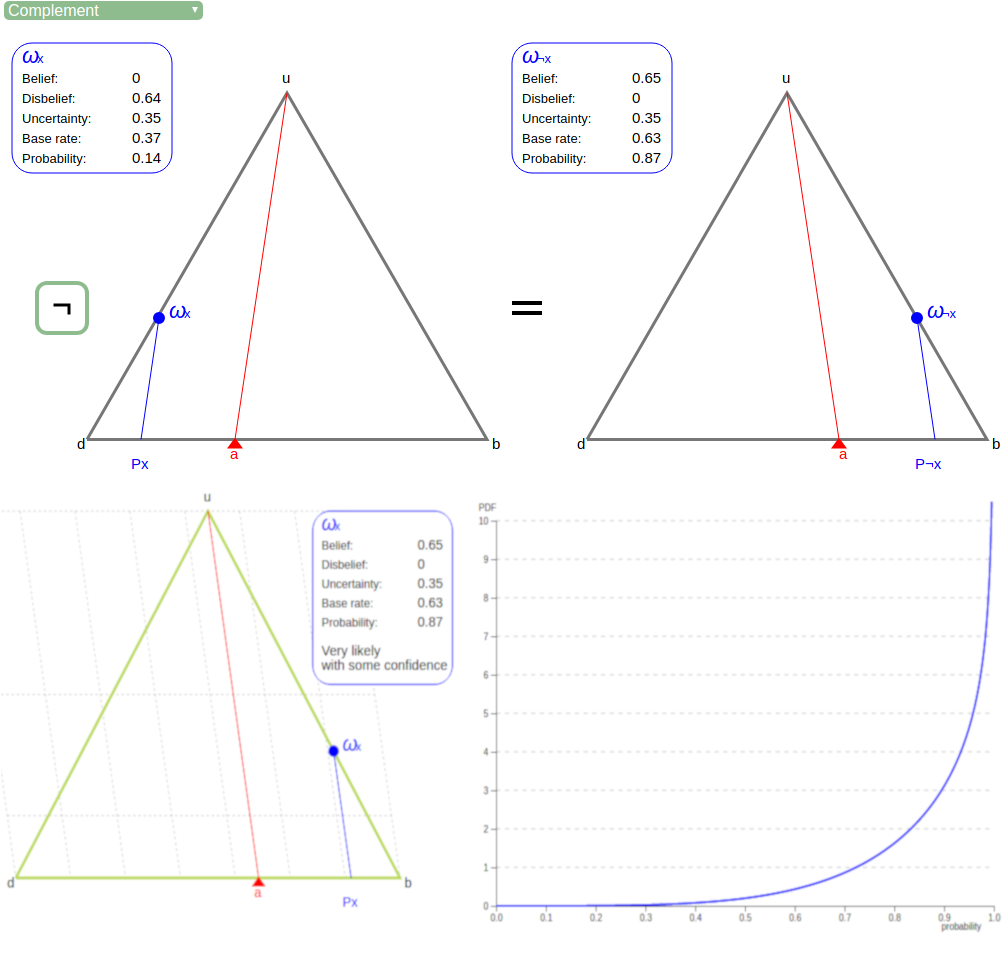
\includegraphics[width=6in]{images/comp1.png}
\end{center}
\needspace{5\baselineskip}
Example 2:
Input data: 
\opinion{x}{0}{0}{1}{0.29}(Vacuous Opinion)
\begin{center}
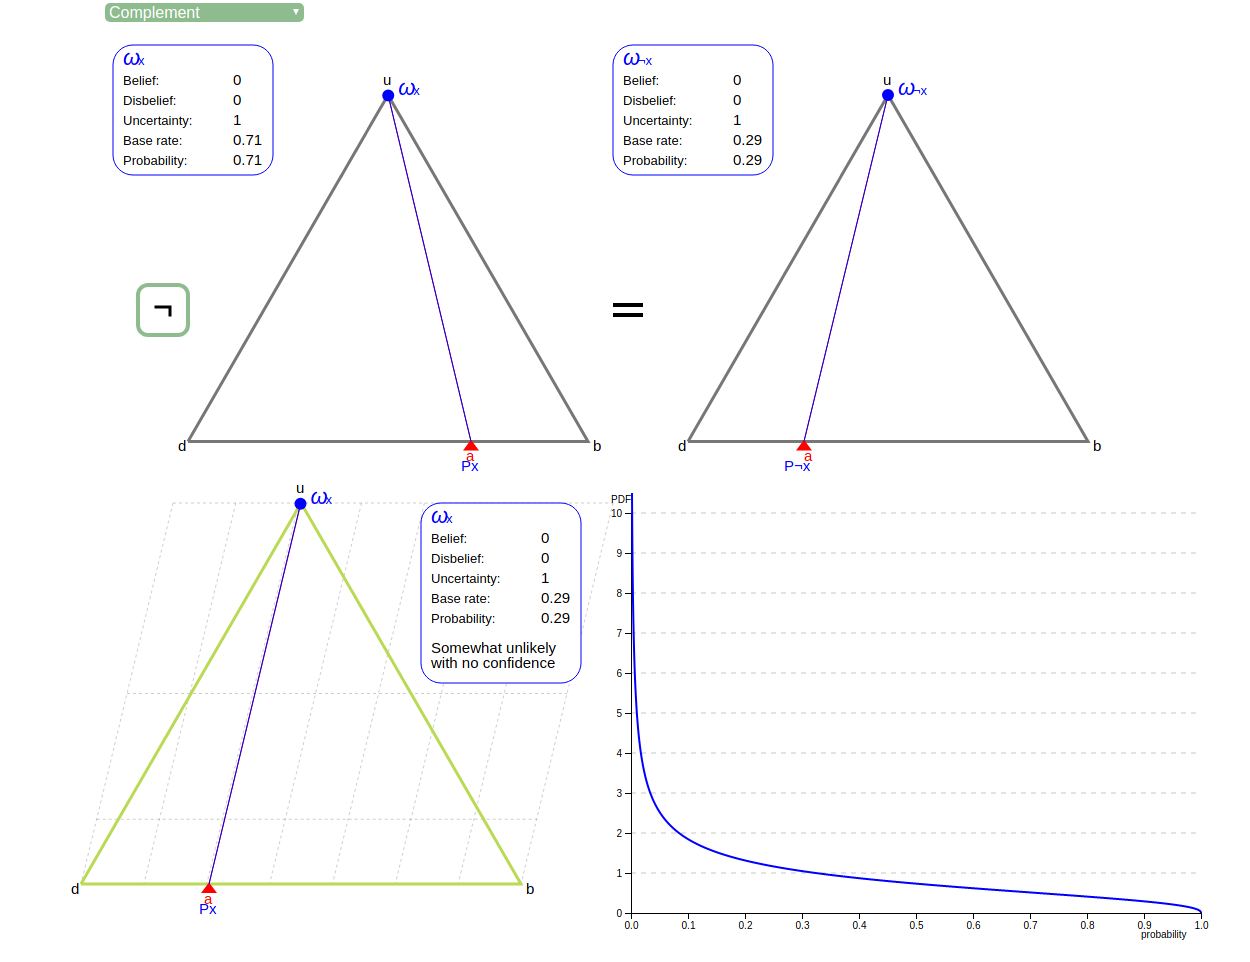
\includegraphics[width=6in]{images/comp2.png}
\end{center}
\subsection{Addition}
Addition of opinions in subjective logic is a binary operator that takes opinions
about two mutually exclusive values (i.e. two disjoint subsets of the same domain)
as arguments, and outputs an opinion about the union of the values.\\
Let \opinion{x_1}{b_{x_1}}{d_{x_1}}{u_{x_1}}{a_{x_1}} and \opinion{x_2}{b_{x_2}}{d_{x_2}}{u_{x_2}}{a_{x_2}} be two binomial opinions. The sum of these two opinions can be expressed as:
$$
\omega_{(x_1 \cup x_2)}: 
\begin{cases}
    b_{(x_1 \cup x_2)} = b_{x_1} + b_{x_2}\\    
    d_{(x_1 \cup x_2)} = \frac{a_{x_1}(d_{x_1} - b_{x_2}) + a_{x_2}(d_{x_2} - b_{x_1})}{a_{x_1} + a_{x_2}}\\
    u_{(x_1 \cup x_2)} = u_x\\
    a_{(x_1 \cup x_2)} = 1 - a_x
\end{cases}
$$\\
Example 1:\\
\begin{center}
    Input data: 
    \opinion{x}{0.16}{0.54}{0.3}{0.73}, 
    \opinion{y}{0.36}{0.21}{0.44}{0.39}\\
    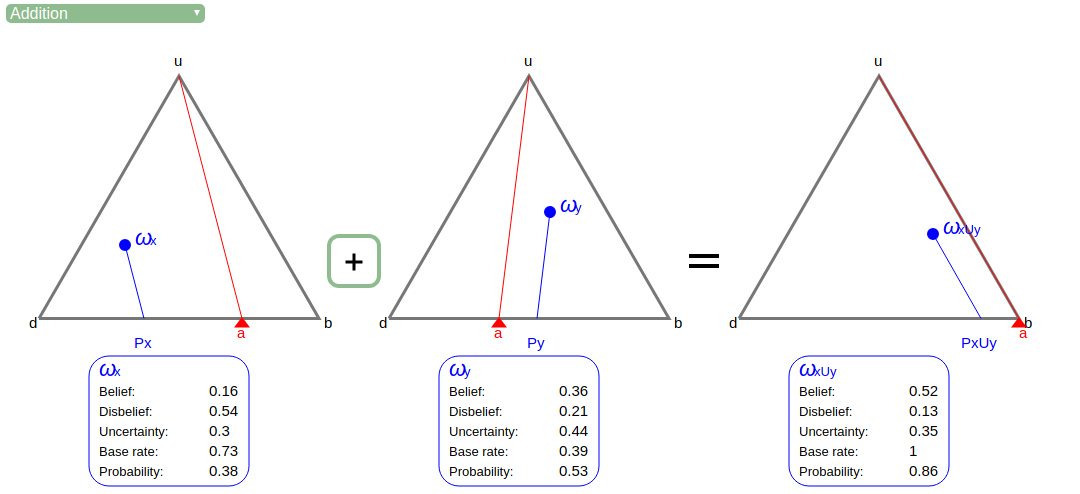
\includegraphics[width=6in]{images/add1.png}
    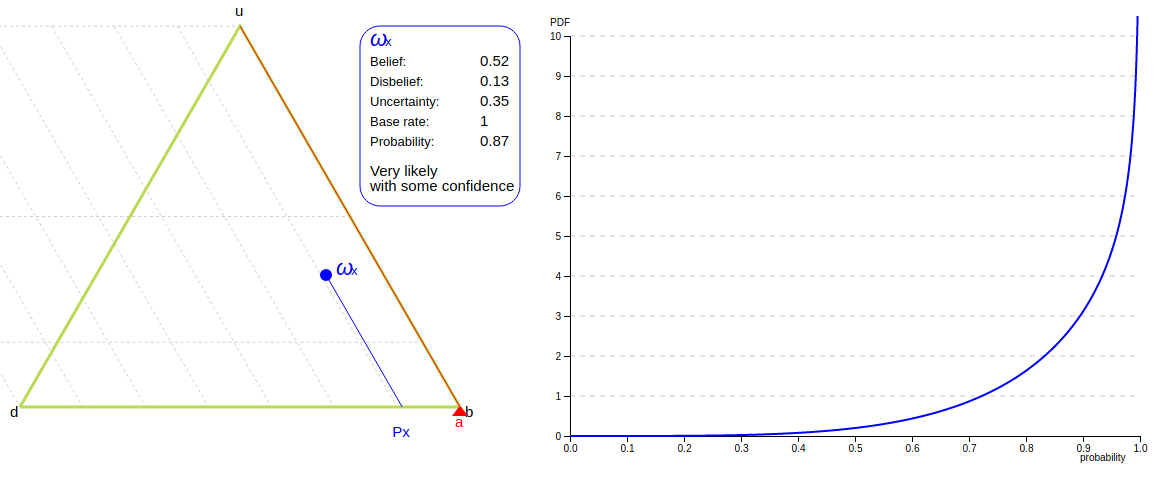
\includegraphics[width=6in]{images/add1viz.png}
\end{center}
\needspace{5\baselineskip}
Example 2:
    \begin{center}
        Input data: 
        \opinion{x}{0}{0}{1}{0.36}, 
        \opinion{y}{0.1}{0.48}{0.43}{0.39}\\
        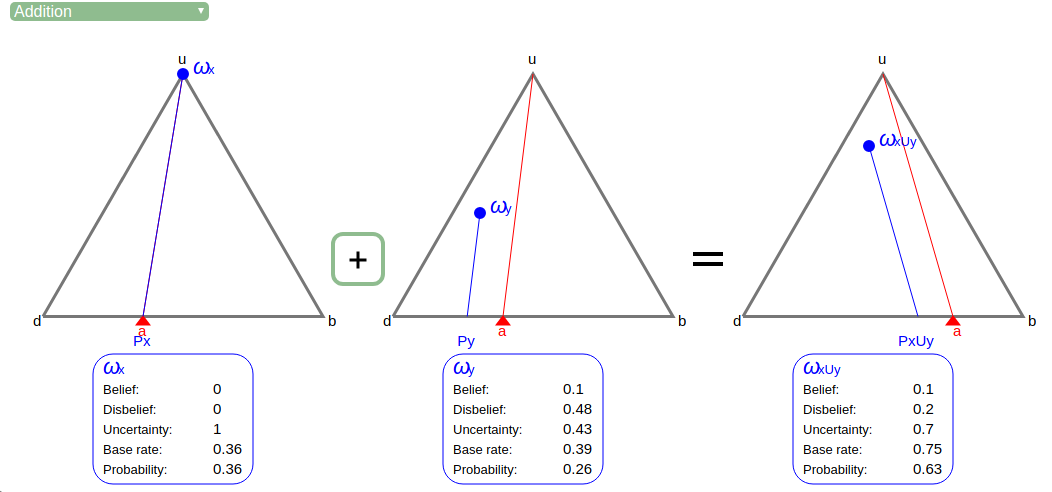
\includegraphics[width=6in]{images/add2.png}
        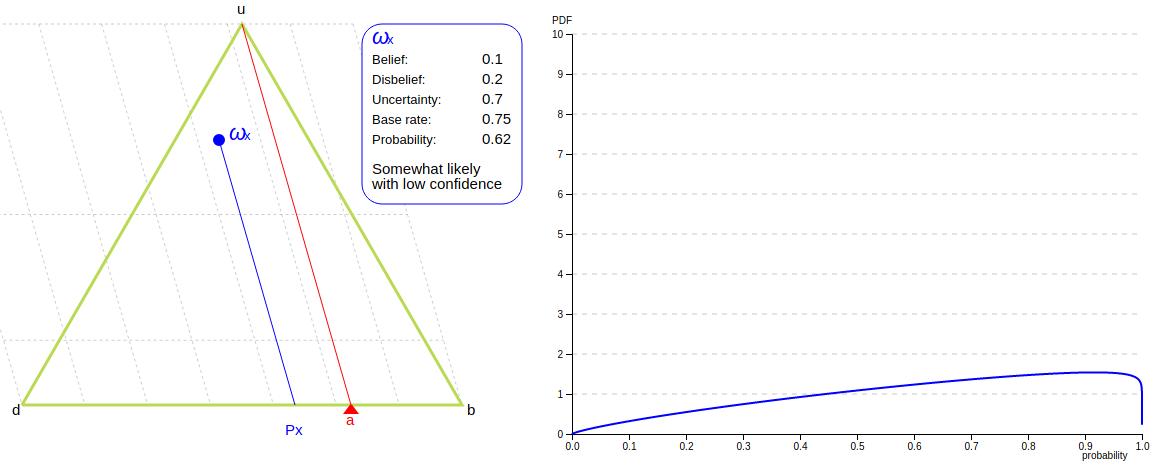
\includegraphics[width=6in]{images/add2viz.png}
    \end{center}
\needspace{5\baselineskip}
Example 3:
    \begin{center}
        Input data: 
        \opinion{x}{0.5}{0.5}{0}{0.36} (Dogmatic), 
        \opinion{y}{0}{0}{1}{0.39} (Vacuous)\\
        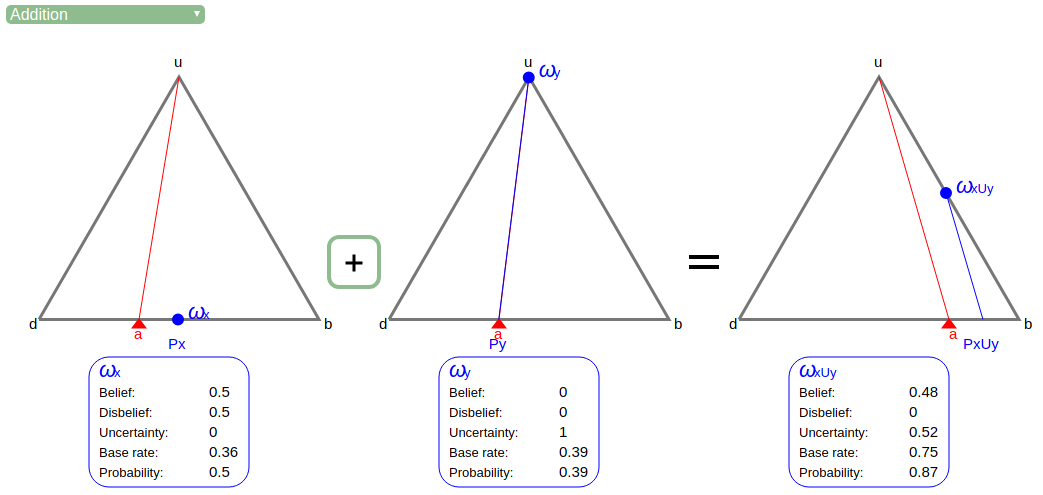
\includegraphics[width=6in]{images/add3.png}
        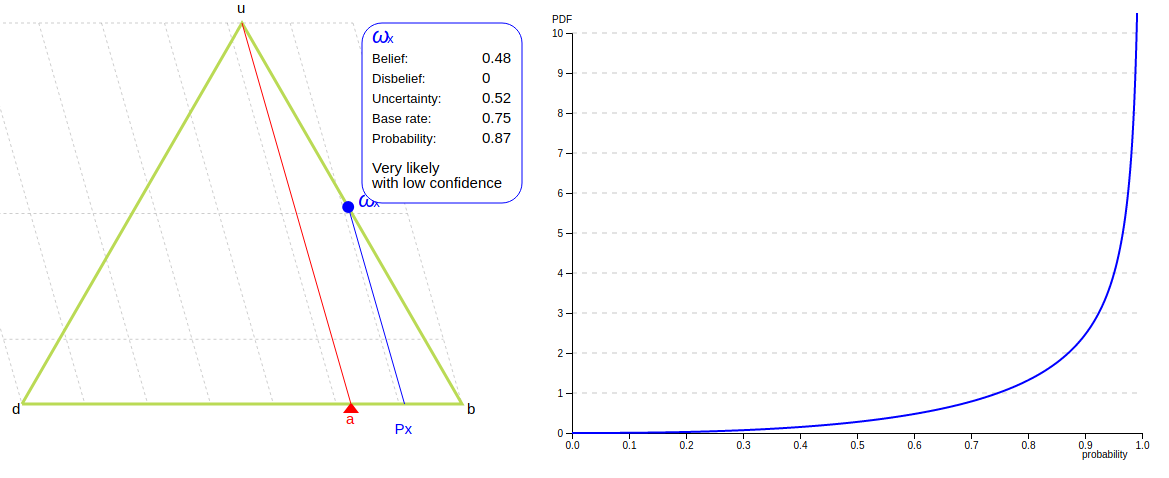
\includegraphics[width=6in]{images/add3viz.png}
    \end{center}

\subsection{Subtraction}
The inverse operation to opinion addition is opinion subtraction. Since addition
of opinions yields the opinion about $x_1 \cup x_2$ from the opinions about disjoint subsets
of the domain, then the difference between the opinions about $x_1 \cup x_2$ and $x_2$ (i.e.
the opinion about $((x_1 \cup x_2)/x_2))$ can only be defined if $x_2 \subseteq (x_1 \cup x_2)$ where $x_2$ and
$(x_1 \cup x_2)$ are subsets of the domain X, i.e. the system must be in the state $(x_1 \cup x_2)$
whenever it is in the state $x_2$. The sum of these two opinions can be expressed as:
$$
\omega_{((x_1 \cup x_2)/x_2)}: 
\begin{cases}
    b_{((x_1 \cup x_2)/x_2)} = b_{(x_1 \cup x_2)} - b_{x_2}\\    
    d_{((x_1 \cup x_2)/x_2)} = \frac{a_{(x_1 \cup x_2)}(d_{(x_1 \cup x_2)} + b_{x_2}) - a_{x_2}(1 + b_{x_2} - b_{(x_1 \cup x_2)} - u_{x_2})}{a_{x_1} + a_{x_2}}\\
    u_{((x_1 \cup x_2)/x_2)} = \frac{a_{(x_1 \cup x_2)} u_{(x_1 \cup x_2)} - a_{x_2} u_{x_2}}{a_{(x_1 \cup x_2)} - a_{x_2}}\\
    a_{((x_1 \cup x_2)/x_2)} = a_{(x_1 \cup x_2)} - a_{x_2}
\end{cases}
$$\\
Example 1:\\
\begin{center}
    Input data: 
    \opinion{x_1 \cup x_2}{0.16}{0.54}{0.3}{0.73}, 
    \opinion{x_2}{0.36}{0.21}{0.44}{0.39}\\
    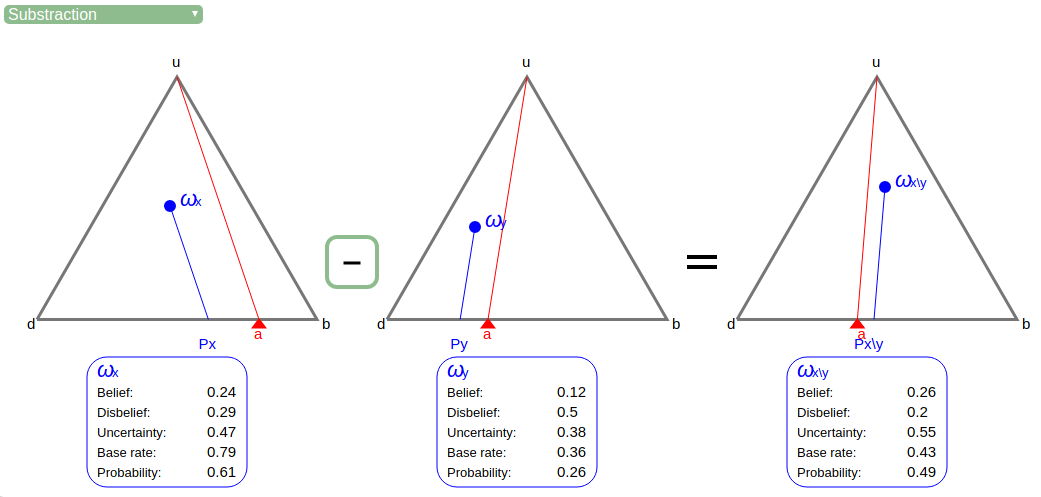
\includegraphics[width=6in]{images/sub1.png}
    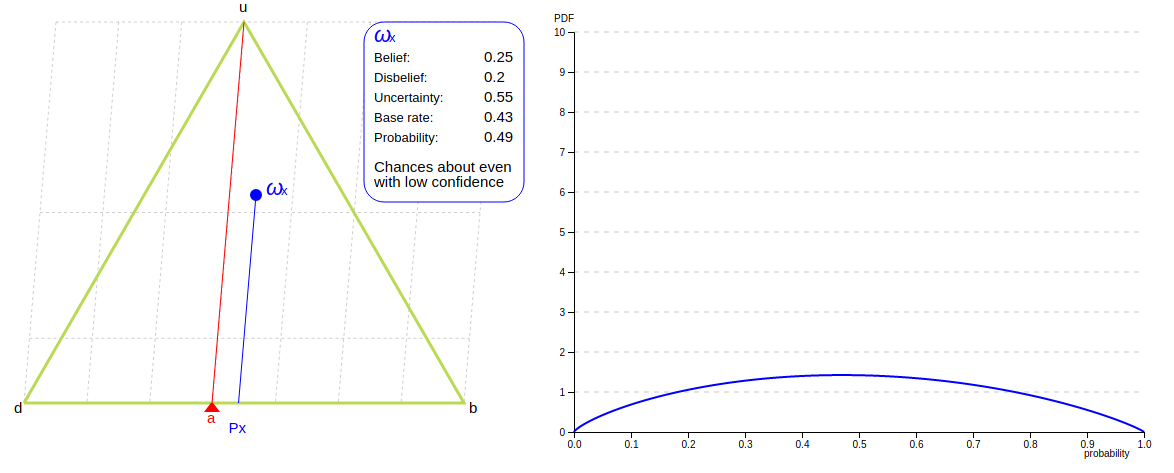
\includegraphics[width=6in]{images/sub1viz.png}
\end{center}
\needspace{5\baselineskip}
Example 2:
    \begin{center}
        Input data: 
        \opinion{x_1 \cup x_2}{0}{0}{1}{0.36}, 
        \opinion{x_2}{0.1}{0.48}{0.43}{0.39}\\
        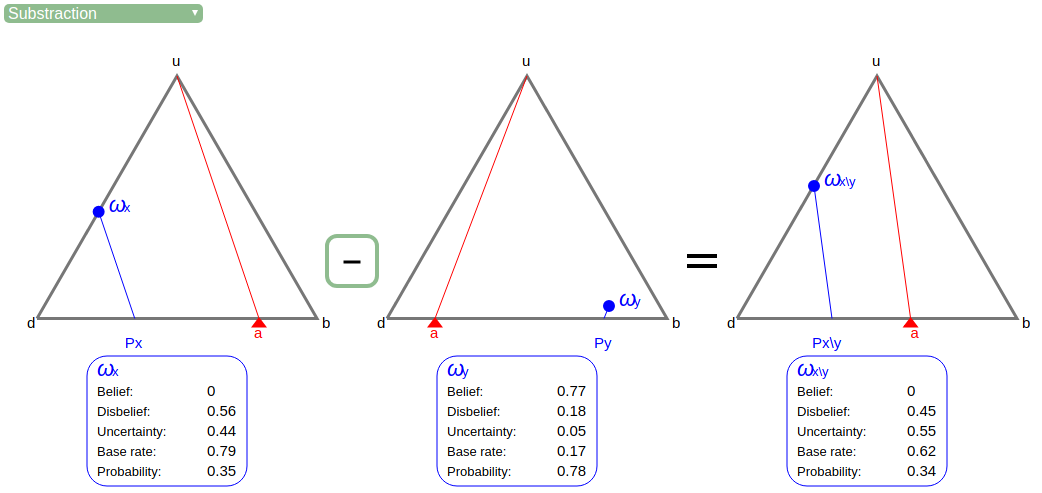
\includegraphics[width=6in]{images/sub2.png}
        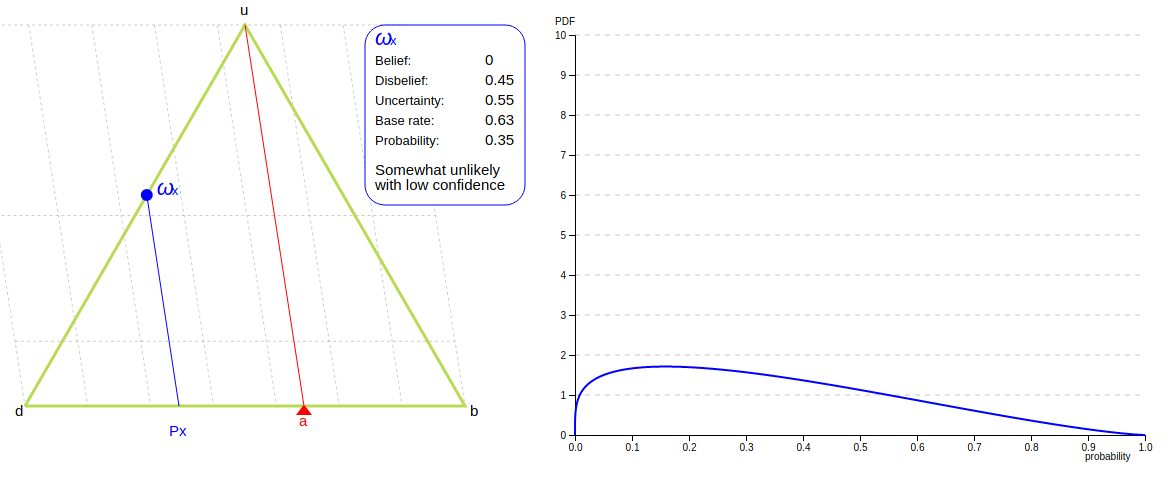
\includegraphics[width=6in]{images/sub2viz.png}
    \end{center}
\needspace{5\baselineskip}
Example 3:
    \begin{center}
        Input data: 
        \opinion{x_1 \cup x_2}{0.5}{0.5}{0}{0.36} (Vacuous), 
        \opinion{x_2}{0}{0}{1}{0.39} (Dogmatic)\\
        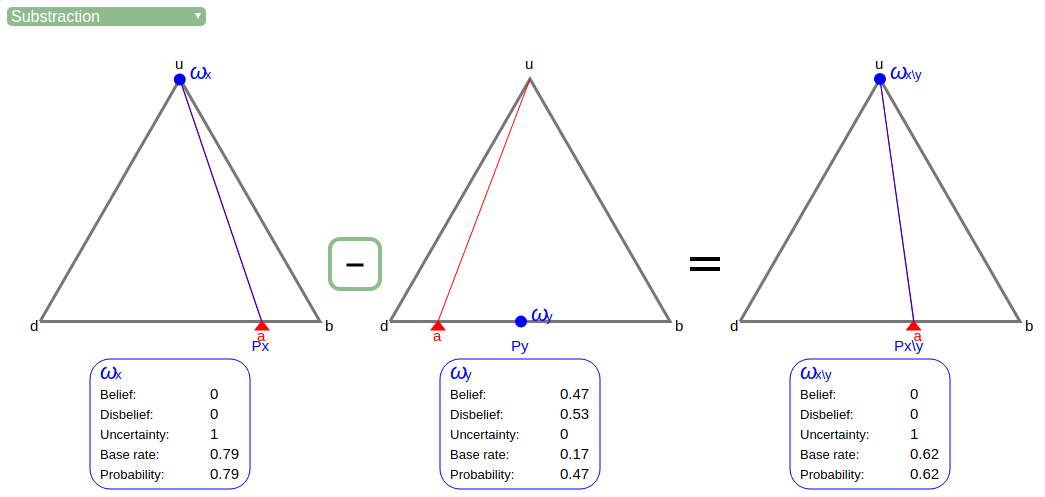
\includegraphics[width=6in]{images/sub3.png}
        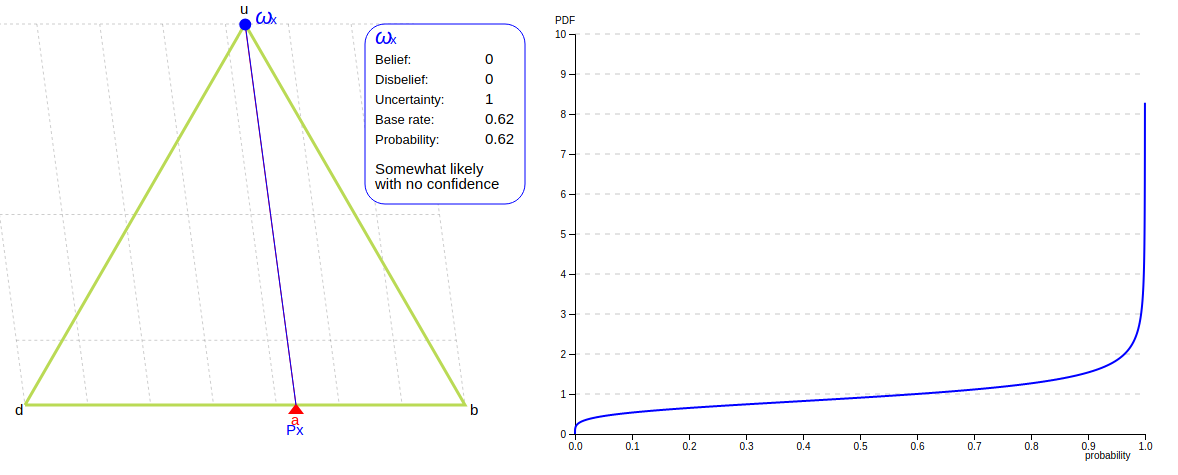
\includegraphics[width=6in]{images/sub3viz.png}
    \end{center}
\end{document}